
%
%    PhD Thesis
% ~~~~~~~~~~~~~~~~~
%  Master Document
%

\documentclass[twoside,openright,12pt]{book}

%  Packages
%***********

\usepackage[utf8]{inputenc}
\usepackage[UKenglish]{babel}
\usepackage[T1]{fontenc}

% Layout
\usepackage{titlesec}
\usepackage{pdfpages}
\usepackage{biblatex}
\usepackage{emptypage}
\usepackage[a4paper]{geometry}
\usepackage{setspace}
\usepackage[garamondx,expert]{mathdesign}
%\usepackage[scaled]{berasans}
%\usepackage[scaled]{beramono}
\usepackage[scaled]{raleway}
\usepackage{textcomp}
\usepackage{tgtermes}
\usepackage{hanging}                      % Used for indented paragraphs
\usepackage{appendix}                     % Added functionality for appendices
\usepackage{fancyhdr}
\usepackage{tocloft}                      % For modifying the Table of Contents

% Text

% Math
\usepackage{nicefrac}
%\usepackage{xfrac}

% Colours
\usepackage{color}
\definecolor{chapter}{gray}{0.6}
\definecolor{appendix}{gray}{0.5}

% Disabled
%~ \usepackage{latexsym}
%~ \usepackage{amsmath}
%~ \usepackage{amssymb}
%~ \usepackage{cite}
%~ \usepackage{graphicx}
%~ \usepackage{float}
%~ \usepackage{listings}
%~ \usepackage{simplewick}
%~ \usepackage{datetime}

% Package Settings
%==================

% Layout
\geometry{twoside,margin=2.5cm}
\renewcommand{\rmdefault}{ptm}
\renewcommand{\sfdefault}{phv}
\renewcommand{\ttdefault}{pcr}
\AtBeginDocument{\parskip=0pt plus 2.5pt\relax\setstretch{1.1}}
\addbibresource{Bibliography.bib}

% Fix section numbering bug in titlesec
\usepackage{etoolbox}
\makeatletter
\patchcmd{\ttlh@hang}{\parindent\z@}{\parindent\z@\leavevmode}{}{}
\patchcmd{\ttlh@hang}{\noindent}{}{}{}
\makeatother

% TOC
\renewcommand\cftpartfont{\sffamily\large}
\renewcommand\cftpartpagefont{\mdseries}
\renewcommand\cftchapfont{\mdseries}
\renewcommand\cftchappagefont{\mdseries}
\renewcommand\cfttoctitlefont{\huge\sffamily}
%\renewcommand{\cftchapleader}{\cftdotfill{\cftdotsep}}

% Custom Commands
%*****************

% Text
\newcommand{\eq}[1]{Eq. \ref{#1}}
\newcommand{\fig}[1]{Fig. \ref{#1}}
\newcommand{\tbl}[1]{Table \ref{#1}}
\newcommand{\ts}[1]{\textsuperscript{#1}}

% Math Commands
\newcommand{\unit}[1]{\,\mathrm{#1}}
\newcommand{\funit}[2]{\,\nicefrac{\mathrm{#1}}{\mathrm{#2}}}
\newcommand{\mexp}[1]{\mathrm{e}^{#1}}
\newcommand{\nexp}[1]{\times 10^{#1}}


% Page Layout
%*************

% Plain Page Numbering
\fancypagestyle{plain}{
    \fancyhf{}
    \fancyfoot[LE,RO]{\thepage}
}

% Header style for numbered chapters
\newcommand{\defaulthead}{
    \fancyhead[LE]{\nouppercase{\itshape\leftmark}}
    \fancyhead[RO]{\nouppercase{\itshape\rightmark}}
}

% Custom heading for unnumbered chapters
\newcommand{\simplehead}[1]{
    \fancyhead[LE]{\nouppercase{\itshape #1}}
    \fancyhead[RO]{\nouppercase{\itshape #1}}
}

\pagestyle{fancy}

% Page Header
\renewcommand{\chaptermark}[1]{\markboth{\chaptername\ \thechapter\ --\ #1}{}}
\renewcommand{\sectionmark}[1]{\markright{\thesection\ #1}{}}
\renewcommand{\headrulewidth}{0pt}
\renewcommand{\footrulewidth}{0pt}

\fancyhf{}
\defaulthead
\headheight 15pt
\fancyfoot[LE,RO]{\thepage}


% Parts
\titleformat{\part}[block]{}{}{}{\centering\fontsize{40}{50}\sffamily}

% Numbered Chapters
\titlespacing*{\chapter}{0mm}{10mm}{20mm}
\titleformat{\chapter}[hang]%
    {\fontsize{60}{70}\sffamily}%
    {\textcolor{chapter}\thechapter}%
    {8mm}%
    {\huge\sffamily}

% Sections
\titleformat{\section}{\large\sffamily}{\thesection}{2mm}{\large}
\titleformat{\subsection}{\normalsize\sffamily}{\thesubsection}{2mm}{}


% Main Document
%***************

\begin{document}

% Front Matters

\frontmatter
    \begin{titlepage}
    \begin{center}
        \vspace*{10mm}
        \huge{}
        Preliminary Title:\\
        Plasma Wakefield Acceleration\\
        \vspace{20mm}
        \large
        \textbf{Veronica K. Berglyd Olsen}\\
        Department of Physics\\
        University of Oslo\\
        Norway\\
        \vfill
        
\includegraphics[width=0.35\textwidth]{images/UiOLogo.pdf}\\
        \vspace{20mm}
        Dissertation Presented for the Degree of\\
        Philosophiae Dpctor (PhD) in Physics\\
        \vspace{10mm}
        \large{July 2017}
    \end{center}
\end{titlepage}

    \chapter*{Abstract}
Abstract

    \chapter*{Acknowledgements}
Acknowledgements

    \tocloftpagestyle{plain}
    \cleardoublepage
    \tableofcontents
    \cleardoublepage

% Main Matters

\pagestyle{fancy}

\mainmatter
    %
%  Introduction
% ==============
%

\chapter{Introduction}
\label{Ch:Intro}

Text

% ================================================================================================ %
\section{Plasma Wakefield Acceleration}
\label{Int:PWFA}

Intro to plasma wakefield goes here

% ================================================================================================ %
\section{Proton Driven Plasma Wakefield Acceleration}
\label{Int:PDPWFA}

Further details on proton driven plasma wakefield goes here.

% ================================================================================================ %
\section{The Self-modulation Instability}
\label{Int:SMI}

Stuff about SMI goes here

% ================================================================================================ %
\section{Numerical Simulations of PWFA}
\label{Int:Sim}

Stuff about Osiris and and all that jazz.

Reference to PIC appendix.

% ================================================================================================ %

    %
%  Wakefield Acceleration
% ========================
%

\chapter{Wakefield Acceleration, an Overview}
\label{Ch:WFA}

Text

% ==================================================================================================================== %
\section{Evolution of the Concept}
\label{WFA:History}

Text

% ==================================================================================================================== %
\section{The Advanced Wakefield Experiment (AWAKE)}
\label{WFA:AWAKE}

Text

% ==================================================================================================================== %
\subsection{AWAKE Run 1}
\label{WFA:AWAKE:R1}

Text

% ==================================================================================================================== %
\subsection{AWAKE Run 2}
\label{WFA:AWAKE:R2}

Text

% ==================================================================================================================== %
\section{The Self-modulation Instability}
\label{WFA:SMI}

Text

% ==================================================================================================================== %
\section{Beam Loading}
\label{WFA:BLoad}

Text

% ==================================================================================================================== %

    %
%  Simulations
% =============
%

\chapter{Simulations}
\label{Ch:Sim}

% ==================================================================================================================== %
\section{Evolution of the Proton Beam}
\label{Sim:PBeam}

Text

% ==================================================================================================================== %
\subsection{Studies with Pre-modulated Beam}
\label{Sim:PBPreMod}

Text

% ==================================================================================================================== %
\subsection{Studies with Single Drive Bunch}
\label{Sim:PBSingle}

Text

% ==================================================================================================================== %
\section{Beam Loading and Energy Spread}
\label{Sim:BLoad}

Text

% ==================================================================================================================== %
\subsection{The Linear Regime}
\label{Sim:Lin}

The ideal case from Tzoufras 2008.

% ==================================================================================================================== %
\subsection{The Quasi-linear Regime}
\label{Sim:QLin}

Text

% ==================================================================================================================== %
\section{Emittance Evolution}
\label{Sim:Emitt}

Emittance is preserved in the linear regime

% ==================================================================================================================== %
\subsection{Beam Matching}
\label{Sim:Match}

Text

% ==================================================================================================================== %
\subsection{The Quasi-linear + Linear Case}
\label{Sim:QLinLin}

Text

% ==================================================================================================================== %
\section{Optimising the Witness Beam}
\label{Sim:Opt}

Bringing it all together.

% ==================================================================================================================== %

    %
%  Summary and Conclusion
% ========================
%

\chapter{Summary and Conclusion}
\label{Ch:SnC}

Text




% Formatting for Appendices and Publications
\titleformat{\chapter}[display]%
    {\Large\sffamily}%
    {\textcolor{appendix}\chaptertitlename\ \textcolor{appendix}\thechapter}%
    {8mm}%
    {\Large\sffamily}

\addtocontents{toc}{\cftpagenumbersoff{part}}

% Appendices

\part*{Appendices}
\appendix
    \chapter{First Appendix}
    Text
    \section{One}
    Section
    \chapter{Second Appendix}
    Text
    \section{One}
    Section

% Publications

\part*{Publications}
\renewcommand\appendixtocname{Publications}
\renewcommand\appendixname{Publication}
\pagestyle{plain}

\appendix
    \renewcommand{\thechapter}{\Roman{chapter}}
    %
%  Publication 1 :: IPAC 2015
% ============================
%

\chapter{Loading of a Plasma-Wakefield Accelerator Section\\
         Driven by a Self-Modulated Proton Bunch}
\label{Pub:IPAC15}

\begin{hangparas}{10mm}{1}

    \textbf{Abstract:}
    We investigate beam loading of a plasma wake driven by a self-modulated proton beam using particle-in-cell
    simulations for phase III of the AWAKE project. We address the case of injection after the proton beam has already
    experienced self-modulation in a previous plasma. Optimal parameters for the injected electron bunch in terms of
    initial beam energy and beam charge density are investigated and evaluated in terms of witness bunch energy and
    energy spread. An approximate modulated proton beam is emulated in order to reduce computation time in these
    simulations.

    \vspace{8mm}

    \textbf{Authors:}
    Veronica K. Berglyd Olsen, Erik Adli (University of Oslo, Oslo, Norway)
    Patric Muggli (Max Planck Institute for Physics, Munich, Germany)
    Ligia D. Amorim, Jorge M. Vieira (Instituto Superior Technico, Lisbon, Portugal)

    \vspace{5mm}

    \textbf{Publication:}
    Proceedings of IPAC 2015, Richmond, Virginia, USA

    \vspace{5mm}

    \textbf{Date:} 3\ts{rd} to 8\ts{th} of May, 2015

\end{hangparas}

    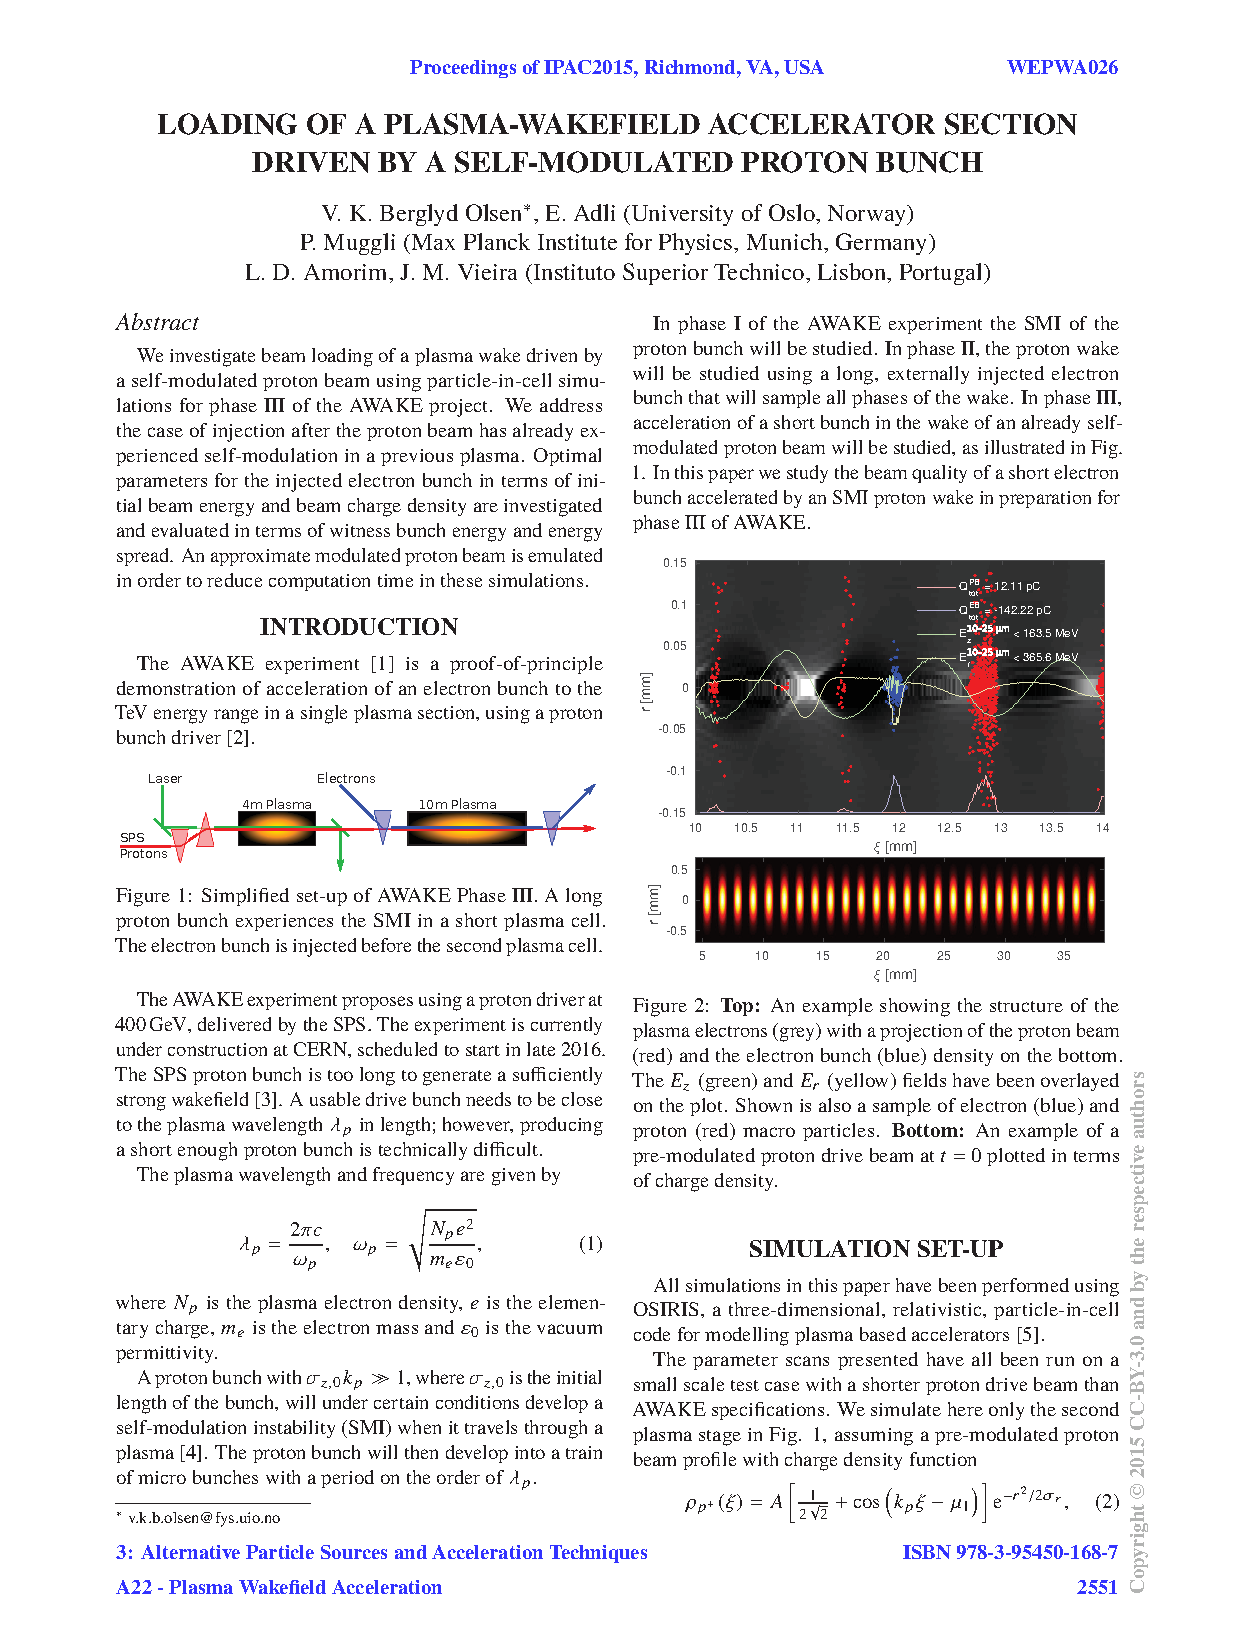
\includepdf[
        pages=1-last,
        openright,
        scale=0.95,
        pagecommand={}
    ]{files/IPAC15-WEPWA026.pdf}
    %
%  Publication 2 :: NAPAC 2016
% =============================
%

\chapter{Loading of Wakefields in a Plasma Accelerator Section\\
         Driven by a Self-Modulated Proton Beam}
\label{Pub:NAPAC16}

\begin{hangparas}{10mm}{1}

    \textbf{Abstract:}
    Using parameters from the AWAKE project and particle-in-cell simulations we investigate beam loading of a plasma wake driven by a self-modulated proton beam. Addressing the case of injection of an electron witness bunch after the drive beam has already experienced self-modulation in a previous plasma, we optimise witness bunch parameters of size, charge and injection phase to maximise energy gain and minimise relative energy spread and emittance of the accelerated bunch.

    \vspace{5mm}

    \textbf{Authors:}
    Veronica K. Berglyd Olsen, Erik Adli (University of Oslo, Oslo, Norway)
    Patric Muggli (Max Planck Institute for Physics, Munich, Germany and CERN, Geneva, Switzerland)
    Jorge M. Vieira (Instituto Superior Technico, Lisbon, Portugal)

    \vspace{5mm}

    \textbf{Publication:}
    Proceedings of NAPAC 2016, Chicago, Illinois, USA

    \vspace{5mm}

    \textbf{Date:} 9\ts{th} to 14\ts{th} of October, 2016


\end{hangparas}

    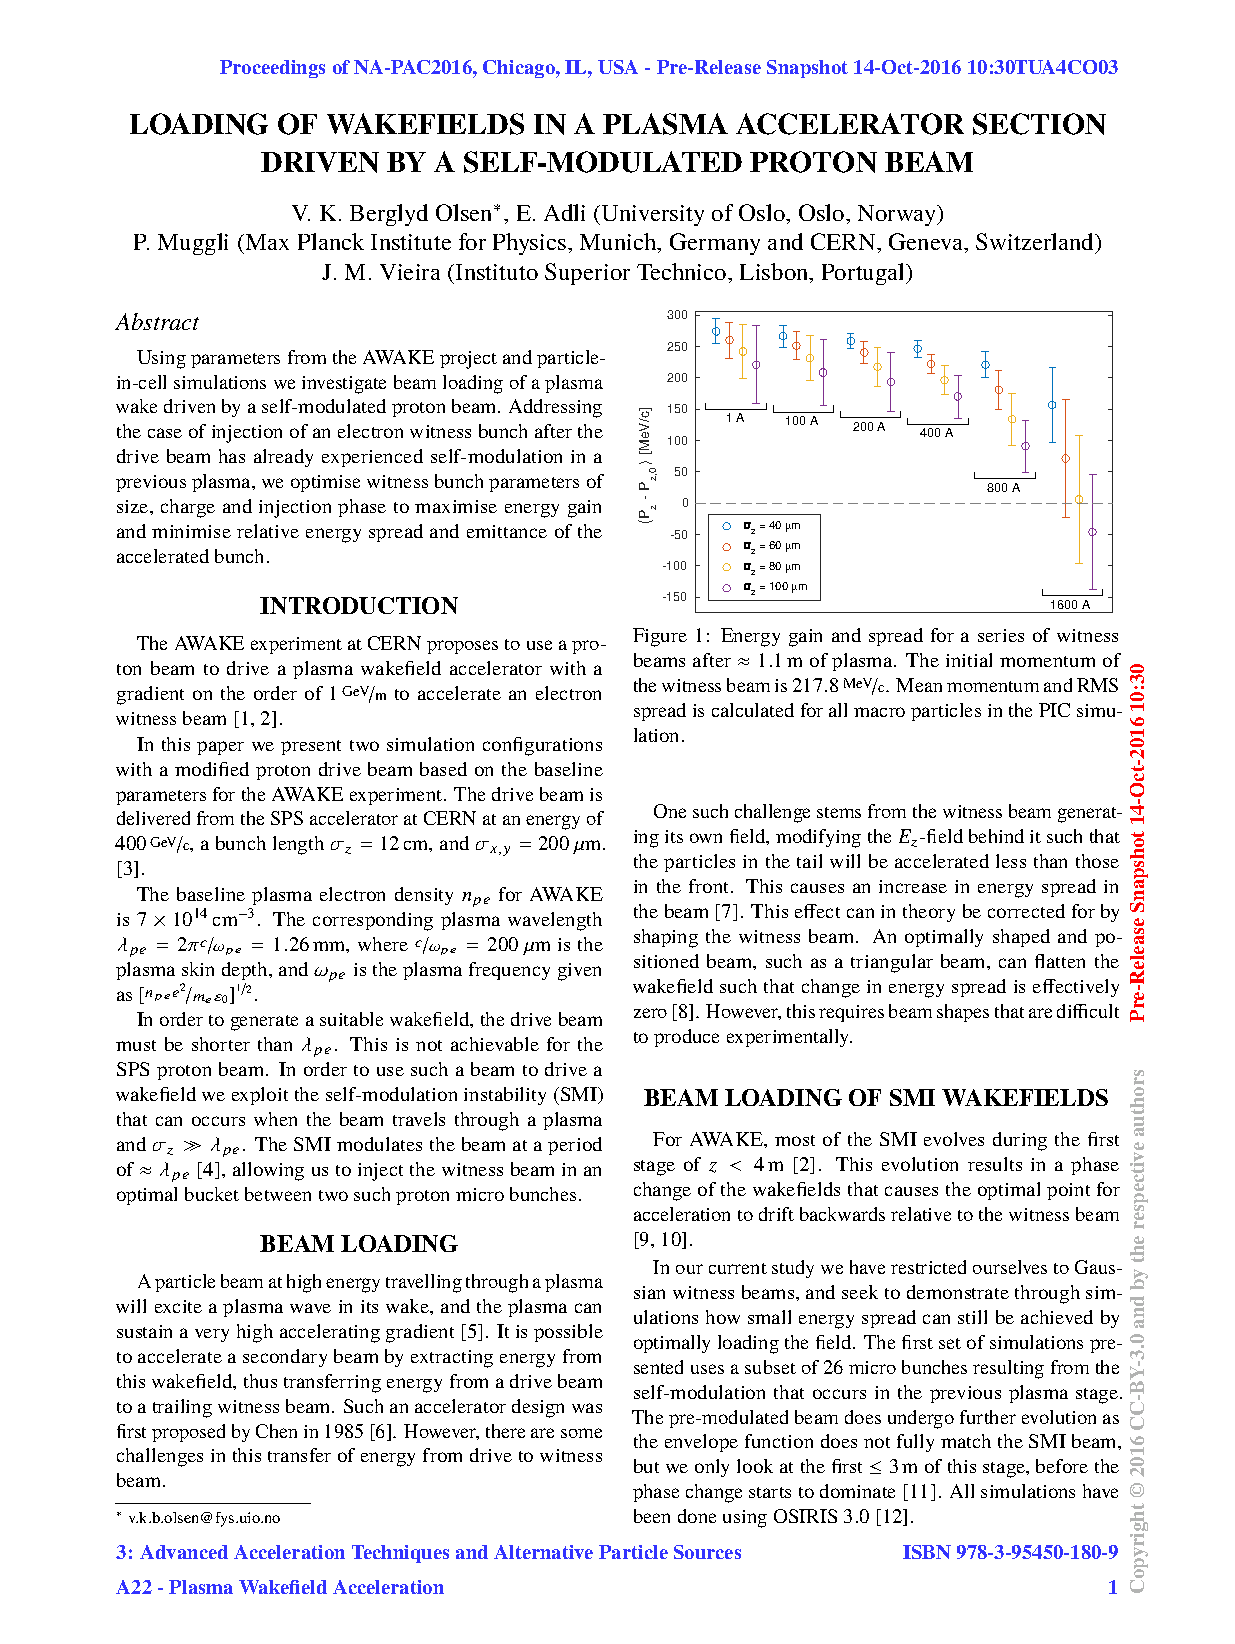
\includepdf[
        pages=1-last,
        openright,
        scale=0.95,
        pagecommand={}
    ]{files/NAPAC16-TUA4CO03.pdf}

% Back Matters

\backmatter
\printbibliography

\end{document}
